
\documentclass[a4paper,12pt]{article}
%%%%%%%%%%%%%%%%%%%%%%%%%%%%%%%%%%%%%%%%%%%%%%%%%%%%%%%%%%%%%%%%%%%%%%%%%%%%%%%%%%%%%%%%%%%%%%%%%%%%%%%%%%%%%%%%%%%%%%%%%%%%%%%%%%%%%%%%%%%%%%%%%%%%%%%%%%%%%%%%%%%%%%%%%%%%%%%%%%%%%%%%%%%%%%%%%%%%%%%%%%%%%%%%%%%%%%%%%%%%%%%%%%%%%%%%%%%%%%%%%%%%%%%%%%%%
\usepackage{eurosym}
\usepackage{vmargin}
\usepackage{amsmath}
\usepackage{graphics}
\usepackage{epsfig}
\usepackage{framed}
\usepackage{subfigure}
\usepackage{fancyhdr}
\usepackage{framed}
\usepackage{subfiles}
\usepackage{graphics}
\usepackage{newlfont}
\usepackage{eurosym}
\usepackage{amsmath,amsthm,amsfonts}
\usepackage{amsmath}
\usepackage{enumerate}
\usepackage{color}
\usepackage{multicol}
\usepackage{amssymb}
\usepackage{multicol}
\usepackage[dvipsnames]{xcolor}
\usepackage{graphicx}

\setcounter{MaxMatrixCols}{10}
%TCIDATA{OutputFilter=LATEX.DLL}
%TCIDATA{Version=5.00.0.2570}
%TCIDATA{<META NAME="SaveForMode"CONTENT="1">}
%TCIDATA{LastRevised=Wednesday, February 23, 201113:24:34}
%TCIDATA{<META NAME="GraphicsSave" CONTENT="32">}
%TCIDATA{Language=American English}

\pagestyle{fancy}
\setmarginsrb{20mm}{0mm}{20mm}{25mm}{12mm}{11mm}{0mm}{11mm}
\lhead{MA4128} \rhead{Kevin O'Brien} \chead{Logistic Regression} %\input{tcilatex}

%http://www.electronics.dit.ie/staff/ysemenova/Opto2/CO_IntroLab.pdf
\begin{document}
	
\section*{Binary Classification}	





\section*{Category Prediction Table}

\begin{itemize}
	\item It is very common to use binomial logistic regression to predict whether cases can be correctly classified (i.e., predicted) from the independent variables. Therefore, it becomes necessary to have a method to assess the effectiveness of the predicted classification against the actual classification.
	\item  There are many methods to assess this with their usefulness oftening depending on the nature of the study conducted. However, all methods revolve around the observed and predicted classifications, which are presented in the ``\texttt{Classification Table}", as shown below:
	
	
	\begin{figure}[h!]
		\centering
		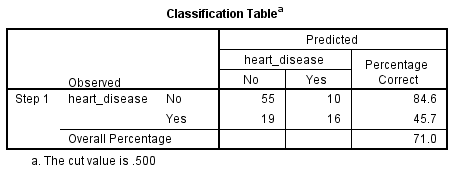
\includegraphics[width=0.8\linewidth]{images/BLogReg-Table}
	\end{figure}
	
	
	
	\item Firstly, notice that the table has a subscript which states, ``\texttt{The cut value is .500}". This means that if the probability of a case being classified into the ``\textbf{\textit{yes}}" category is greater than .500, then that particular case is classified into the ``\textbf{\textit{yes}}" category. 
	Otherwise, the case is classified as in the ``\textbf{\textit{no}}" category. 
\end{itemize}



\subsection*{Classification Table}
\begin{itemize}
\item Rather than using a goodness-of-fit statistic, we often want to look at the proportion of cases we have managed to classify correctly. For this we need to look at the classification table printed out by SPSS, which tells us how many of the cases where the observed values of the dependent variable were 1 or 0 respectively have
been correctly predicted.
\item 
In the Classification table, the columns are the two predicted values of the dependent, while the rows are the two observed (actual) values of the dependent. In a perfect model, all cases will be on the diagonal and the
overall percent correct will be 100\%. 
\item In this study, 87.5\% were correctly classified for the take offer group and 92.9\% for the decline offer group. Overall 90\% were correctly classified. This is a considerable improvement on the 53.3\% correct classification with the constant model so we know that the model with predictors is a significantly better mode.
\end{itemize}
\begin{figure}[h!]
	\begin{center}
		% Requires \usepackage{graphicx}
		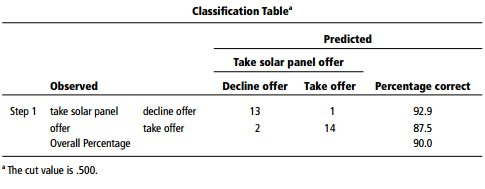
\includegraphics[scale=0.8]{images/Logistic7}\\
		%\caption{Classification Table}
	\end{center}
\end{figure}

\subsection*{Classification Plot} 
The classification plot or histogram of predicted probabilities
provides a visual demonstration of the correct and incorrect predictions. Also called the `\texttt{classplot}' or the `\texttt{plot of observed groups and predicted probabilities}, it is another very useful piece of information from the SPSS output when one chooses
\texttt{Classification plots}' under the Options button in the Logistic Regression dialogue box.

\subsection*{Interpreting the Classifcation Table}
Whilst the classification table appears to be very simple, it actually provides a lot of important information about your binomial logistic regression result, including:


\begin{itemize}
	\item[A.] The \textbf{percentage accuracy in classification (PAC)}, which reflects the percentage of cases that can be correctly classified as "no" heart disease with the independent variables added (not just the overall model).
	\item[B.] \textbf{Sensitivity}, which is the percentage of cases that had the observed characteristic (e.g., "yes" for heart disease) which were correctly predicted by the model (i.e., true positives).
	\item[C.] \textbf{Specificity}, which is the percentage of cases that did not have the observed characteristic (e.g., "no" for heart disease) and were also correctly predicted as not having the observed characteristic (i.e., true negatives).
	\item[D.] The \textbf{positive predictive value}, which is the percentage of correctly predicted cases ``with" the observed characteristic compared to the total number of cases predicted as having the characteristic.
	\item[E.] The \textbf{negative predictive value}, which is the percentage of correctly predicted cases ``without" the observed characteristic compared to the total number of cases predicted as not having the characteristic.
\end{itemize}
%--------------------------------------------------------------------------------------%

\newpage


	
\section*{SPSS Output}
The variable \textbf{\textit{Vote2005}} is a binary variable describing turnout at a general election. The predictor variables are gender and age.
\begin{center}
	\begin{figure}[h!]
		% Requires \usepackage{graphicx}
		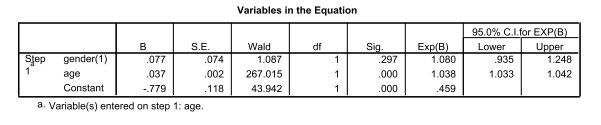
\includegraphics[scale=0.8]{images/LogWeek10B.jpg}\\
		%\caption{General Election 2005}
	\end{figure}
\end{center}
\vspace{-1.7cm}
\[\mbox{logit(vote2005)} = -0.779 + 0.077\mbox{gender(1)}+0.037\mbox{age}\]
\begin{itemize}
	\item The age coefficient is statistically significant. The odds ratio (``Exp(B)") for age is 1.038, which
	means for each year different in age, the person is 1.038 times more likely to turn
	out to vote, having allowed for gender in the model. 
	\item For example, a 21 year old is 1.038
	times as likely to turn out to vote than a 20 year old. This might not seem much
	of a difference but a 20 year difference leads to a person being $1.038^20 = 2.11$
	times more likely to turn out to vote. 
	\item  A 40 year old is 2.11 times more likely to
	turn out to vote than a 20 year old, having allowed for gender in the model.
	\item The gender variable has been turned into a binary variable. The default setting for gender ("0") is for female voters. The gender coefficient is not statistically significant. 
\end{itemize}




\end{document}